Le projet est pré-déployé sur la machine virtuelle (VM) fournie. 

Identifiant de la VM : 
\begin{itemize}[label=$\bullet$]
	\item Nom d'utilisateur: adminN0L
	\item Mot de passe: adminN0L
\end{itemize}

Un raccourci "prj2324.local" est présent sur le bureau pour accéder au site web. Wamp64 doit être démarré pour accéder au site.

Voici les étapes réalisées pour le déploiement:

\begin{enumerate}
	\item Installation de Wamp64 Server (PHP 8.2)
	\begin{itemize}[label=$\bullet$]
		\item \url{https://www.wampserver.com/en/download-wampserver-64bits/}
	\end{itemize}
	
	\item Installation de DBeaver afin de facilité la gestion de la base de données. Il n'est cependant pas nécessaire au bon fonctionnement du site. C'est via celui-ci que j'ai importé le \textit{\url{prj2324.sql}}
	\begin{itemize}[label=$\bullet$]
		\item \url{https://dbeaver.io/}
	\end{itemize}
	
	\item PhpStorm est présent sur la VM, il n'est pas du tout requis au bon fonctionnement du site. Il est uniquement présent afin de faciliter votre navigation dans le code source.

	\item Le code source du site web est présent dans le répertoire suivant :
	\begin{itemize}[label=$\bullet$]
		\item \url{C:\wamp64\www\HanutA\_PrjDevWeb2324-master}
	\end{itemize}
		
	\newpage
	\item Créer le virtual host sur Wamp64 : dans ce cas, le lien vers le projet sera : \\ \url{http://prj2324.local}
	\begin{figure}[h]
		\centering
		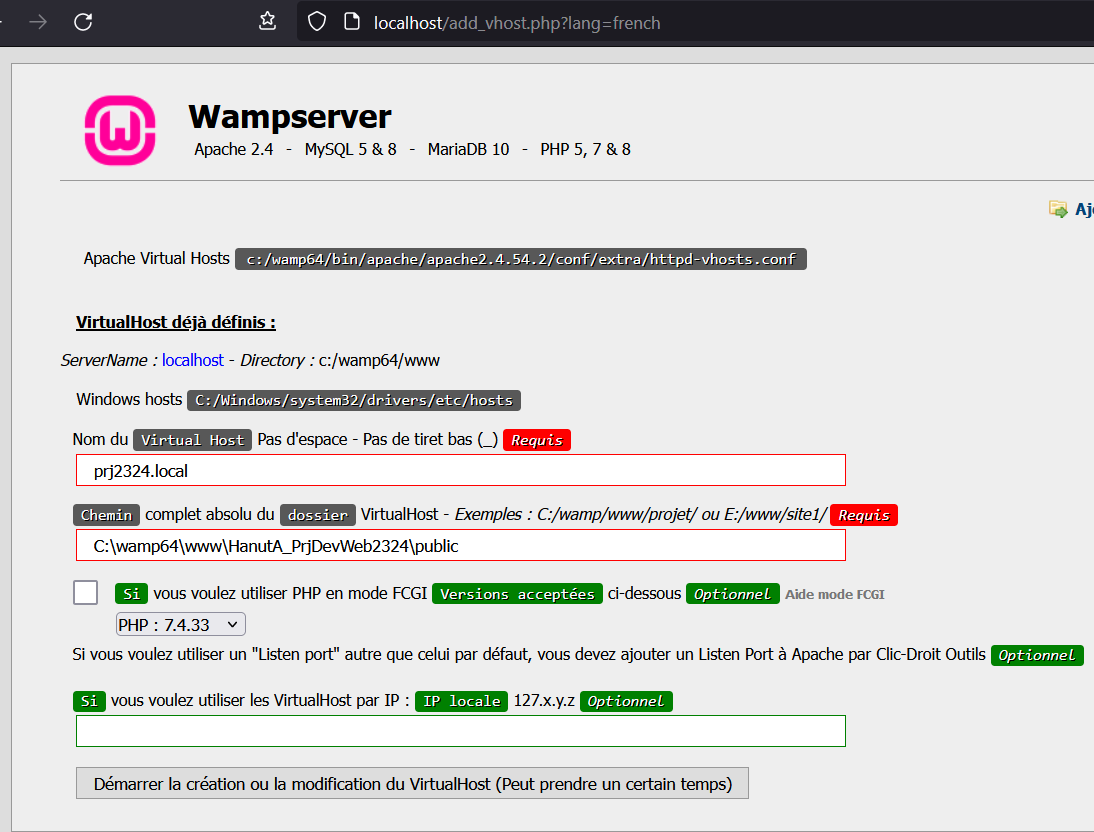
\includegraphics[keepaspectratio,width=15cm]{images/VirtualHost}
		\caption{Interface de création d'un VirtualHost via Wamp64}
	\end{figure}
\end{enumerate}